\refstepcounter{section}
\section*{Lecture 28: Introduction to RG}
\addcontentsline{toc}{section}{Lecture 28: Introduction to RG}
We will have a sketchy introduction to the enlightening concept of the \textit{renormalisation group}. RG can explain universality (why vastly different models seem to have same critical exponents ) and can also predict these exponents. RG is an approach to approximately calculate the sums involved in the partition function. \\[0.2cm]
Renormalisation basically means doing certain transformations or reparameterisation, in the hope that it will make the theory easier. It is called `group' since two such transformations leads to a third transformation (composition rule). 
First let us use this for the 1D Ising model. Consider $N$ Ising spins on a 1D lattice with periodic boundary condition (\textit{i.e.} $\sigma_1 \equiv \sigma_{N+1}$) with the following Hamiltonian,
$$\SH = -J \sum\limits_{i=1}^N \sigma_i \sigma_{i+1}$$
For this case, we take the zero field condition. We define $K := \beta J$ and using this, the partition function becomes, 
$$\SZ = \sum\limits_{\sigma_1 = \pm 1}\sum\limits_{\sigma_2 = \pm 1}\cdots \sum\limits_{\sigma_N = \pm 1} e^{K\sum_i \sigma_i \sigma_{i+1}} \equiv \sum\limits_{\sigma_1 = \pm 1}\sum\limits_{\sigma_2 = \pm 1}\cdots \sum\limits_{\sigma_N = \pm 1} e^{K\qty(\sigma_1 \sigma_2 + \sigma_2\sigma_3 + \sigma_3\sigma_4 \ldots \sigma_N\sigma_1)}$$
Note that the even spins, say $\sigma_2$, appears in two consecutive terms. We can first do the trace over the even spins then, which gives us, 
\begin{align}
    \begin{split}
        \SZ &= \sum\limits_{\sigma_1 = \pm 1}\sum\limits_{\sigma_3 = \pm 1}\sum\limits_{\sigma_5 = \pm 1}\cdots \sum\limits_{\sigma_N = \pm 1} \prod\limits_{j=1}^{N/2} \qty(e^{K \qty(\sigma_{2j-1}+\sigma_{2j+1})}+e^{-K \qty(\sigma_{2j-1}+\sigma_{2j+1})})\\
&\equiv \sum\limits_{\sigma_1 = \pm 1}\sum\limits_{\sigma_3 = \pm 1}\sum\limits_{\sigma_5 = \pm 1}\cdots \sum\limits_{\sigma_N = \pm 1} \prod\limits_{j=1}^{N/2} \qty[2\cosh(K \qty(\sigma_{2j-1}+\sigma_{2j+1}))]
    \end{split}
\end{align}
Next, if we assume that there exist some function $f(K)$ and $K'$ such that \begin{equation}\label{coshspin}
    2\cosh(K \qty(\sigma_{2j-1}+\sigma_{2j+1})) = f(K)e^{K'\sigma_{2j-1}\sigma_{2j+1}}\qquad \forall\ j 
\end{equation}
then the partition function will take the following form, 
\begin{align}
        \SZ =(f(K))^{N/2} \mathcolor{red}{\sum\limits_{\sigma_1 = \pm 1}\sum\limits_{\sigma_3 = \pm 1}\sum\limits_{\sigma_5 = \pm 1}\cdots \sum\limits_{\sigma_N = \pm 1} \prod\limits_{j=1}^{N/2}  e^{K'\sigma_{2j-1}\sigma_{2j+1}}}
\end{align}
If we forgo the indexing, the red colour is exactly the partition function for a 1D Ising chain with $N/2$ spins and coupling constant $K'$. Thus, the partition function with $N$ spins and coupling $K$ follows, 
\begin{equation}\label{partition}
    \SZ\tund{N}(K) = (f(K))^{N/2} \SZ\tund{N/2}(K')
\end{equation}
\begin{figure}[H]
    \centering 
    

\tikzset{every picture/.style={line width=0.75pt}} %set default line width to 0.75pt        

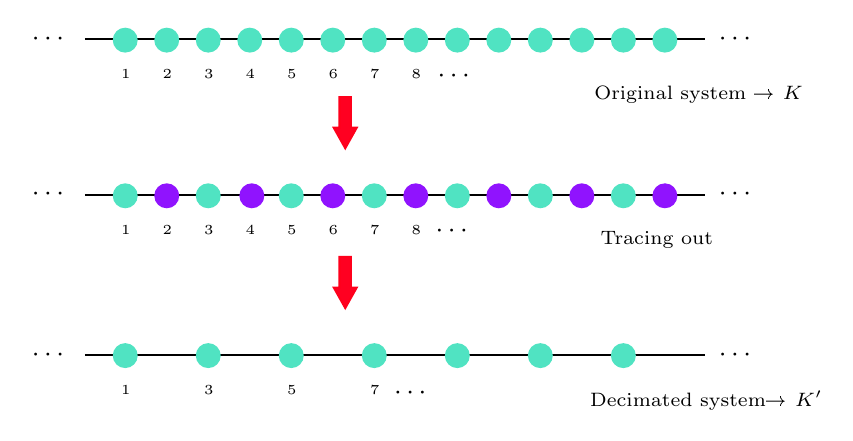
\begin{tikzpicture}[x=0.75pt,y=0.75pt,yscale=-1,xscale=1]
%uncomment if require: \path (0,332); %set diagram left start at 0, and has height of 332

%Straight Lines [id:da156253805786725] 
\draw    (121,110) -- (420,110) ;
%Shape: Circle [id:dp3032403975950799] 
\draw  [color={rgb, 255:red, 80; green, 227; blue, 194 }  ,draw opacity=1 ][fill={rgb, 255:red, 80; green, 227; blue, 194 }  ,fill opacity=1 ] (135,110.5) .. controls (135,107.46) and (137.46,105) .. (140.5,105) .. controls (143.54,105) and (146,107.46) .. (146,110.5) .. controls (146,113.54) and (143.54,116) .. (140.5,116) .. controls (137.46,116) and (135,113.54) .. (135,110.5) -- cycle ;
%Shape: Circle [id:dp8768516051634454] 
\draw  [color={rgb, 255:red, 80; green, 227; blue, 194 }  ,draw opacity=1 ][fill={rgb, 255:red, 80; green, 227; blue, 194 }  ,fill opacity=1 ] (155,110.5) .. controls (155,107.46) and (157.46,105) .. (160.5,105) .. controls (163.54,105) and (166,107.46) .. (166,110.5) .. controls (166,113.54) and (163.54,116) .. (160.5,116) .. controls (157.46,116) and (155,113.54) .. (155,110.5) -- cycle ;
%Shape: Circle [id:dp9649738041870417] 
\draw  [color={rgb, 255:red, 80; green, 227; blue, 194 }  ,draw opacity=1 ][fill={rgb, 255:red, 80; green, 227; blue, 194 }  ,fill opacity=1 ] (175,110.5) .. controls (175,107.46) and (177.46,105) .. (180.5,105) .. controls (183.54,105) and (186,107.46) .. (186,110.5) .. controls (186,113.54) and (183.54,116) .. (180.5,116) .. controls (177.46,116) and (175,113.54) .. (175,110.5) -- cycle ;
%Shape: Circle [id:dp6833438757398491] 
\draw  [color={rgb, 255:red, 80; green, 227; blue, 194 }  ,draw opacity=1 ][fill={rgb, 255:red, 80; green, 227; blue, 194 }  ,fill opacity=1 ] (195,110.5) .. controls (195,107.46) and (197.46,105) .. (200.5,105) .. controls (203.54,105) and (206,107.46) .. (206,110.5) .. controls (206,113.54) and (203.54,116) .. (200.5,116) .. controls (197.46,116) and (195,113.54) .. (195,110.5) -- cycle ;
%Shape: Circle [id:dp2607812925995878] 
\draw  [color={rgb, 255:red, 80; green, 227; blue, 194 }  ,draw opacity=1 ][fill={rgb, 255:red, 80; green, 227; blue, 194 }  ,fill opacity=1 ] (215,110.5) .. controls (215,107.46) and (217.46,105) .. (220.5,105) .. controls (223.54,105) and (226,107.46) .. (226,110.5) .. controls (226,113.54) and (223.54,116) .. (220.5,116) .. controls (217.46,116) and (215,113.54) .. (215,110.5) -- cycle ;
%Shape: Circle [id:dp5548764367024854] 
\draw  [color={rgb, 255:red, 80; green, 227; blue, 194 }  ,draw opacity=1 ][fill={rgb, 255:red, 80; green, 227; blue, 194 }  ,fill opacity=1 ] (235,110.5) .. controls (235,107.46) and (237.46,105) .. (240.5,105) .. controls (243.54,105) and (246,107.46) .. (246,110.5) .. controls (246,113.54) and (243.54,116) .. (240.5,116) .. controls (237.46,116) and (235,113.54) .. (235,110.5) -- cycle ;
%Shape: Circle [id:dp24108252785685447] 
\draw  [color={rgb, 255:red, 80; green, 227; blue, 194 }  ,draw opacity=1 ][fill={rgb, 255:red, 80; green, 227; blue, 194 }  ,fill opacity=1 ] (255,110.5) .. controls (255,107.46) and (257.46,105) .. (260.5,105) .. controls (263.54,105) and (266,107.46) .. (266,110.5) .. controls (266,113.54) and (263.54,116) .. (260.5,116) .. controls (257.46,116) and (255,113.54) .. (255,110.5) -- cycle ;
%Shape: Circle [id:dp7626307281526219] 
\draw  [color={rgb, 255:red, 80; green, 227; blue, 194 }  ,draw opacity=1 ][fill={rgb, 255:red, 80; green, 227; blue, 194 }  ,fill opacity=1 ] (275,110.5) .. controls (275,107.46) and (277.46,105) .. (280.5,105) .. controls (283.54,105) and (286,107.46) .. (286,110.5) .. controls (286,113.54) and (283.54,116) .. (280.5,116) .. controls (277.46,116) and (275,113.54) .. (275,110.5) -- cycle ;
%Shape: Circle [id:dp4766135164306231] 
\draw  [color={rgb, 255:red, 80; green, 227; blue, 194 }  ,draw opacity=1 ][fill={rgb, 255:red, 80; green, 227; blue, 194 }  ,fill opacity=1 ] (295,110.5) .. controls (295,107.46) and (297.46,105) .. (300.5,105) .. controls (303.54,105) and (306,107.46) .. (306,110.5) .. controls (306,113.54) and (303.54,116) .. (300.5,116) .. controls (297.46,116) and (295,113.54) .. (295,110.5) -- cycle ;
%Shape: Circle [id:dp27190659026917463] 
\draw  [color={rgb, 255:red, 80; green, 227; blue, 194 }  ,draw opacity=1 ][fill={rgb, 255:red, 80; green, 227; blue, 194 }  ,fill opacity=1 ] (315,110.5) .. controls (315,107.46) and (317.46,105) .. (320.5,105) .. controls (323.54,105) and (326,107.46) .. (326,110.5) .. controls (326,113.54) and (323.54,116) .. (320.5,116) .. controls (317.46,116) and (315,113.54) .. (315,110.5) -- cycle ;
%Shape: Circle [id:dp8401954201976427] 
\draw  [color={rgb, 255:red, 80; green, 227; blue, 194 }  ,draw opacity=1 ][fill={rgb, 255:red, 80; green, 227; blue, 194 }  ,fill opacity=1 ] (335,110.5) .. controls (335,107.46) and (337.46,105) .. (340.5,105) .. controls (343.54,105) and (346,107.46) .. (346,110.5) .. controls (346,113.54) and (343.54,116) .. (340.5,116) .. controls (337.46,116) and (335,113.54) .. (335,110.5) -- cycle ;
%Shape: Circle [id:dp3305949675677218] 
\draw  [color={rgb, 255:red, 80; green, 227; blue, 194 }  ,draw opacity=1 ][fill={rgb, 255:red, 80; green, 227; blue, 194 }  ,fill opacity=1 ] (355,110.5) .. controls (355,107.46) and (357.46,105) .. (360.5,105) .. controls (363.54,105) and (366,107.46) .. (366,110.5) .. controls (366,113.54) and (363.54,116) .. (360.5,116) .. controls (357.46,116) and (355,113.54) .. (355,110.5) -- cycle ;
%Shape: Circle [id:dp5069635166107922] 
\draw  [color={rgb, 255:red, 80; green, 227; blue, 194 }  ,draw opacity=1 ][fill={rgb, 255:red, 80; green, 227; blue, 194 }  ,fill opacity=1 ] (375,110.5) .. controls (375,107.46) and (377.46,105) .. (380.5,105) .. controls (383.54,105) and (386,107.46) .. (386,110.5) .. controls (386,113.54) and (383.54,116) .. (380.5,116) .. controls (377.46,116) and (375,113.54) .. (375,110.5) -- cycle ;
%Shape: Circle [id:dp5821934865777897] 
\draw  [color={rgb, 255:red, 80; green, 227; blue, 194 }  ,draw opacity=1 ][fill={rgb, 255:red, 80; green, 227; blue, 194 }  ,fill opacity=1 ] (395,110.5) .. controls (395,107.46) and (397.46,105) .. (400.5,105) .. controls (403.54,105) and (406,107.46) .. (406,110.5) .. controls (406,113.54) and (403.54,116) .. (400.5,116) .. controls (397.46,116) and (395,113.54) .. (395,110.5) -- cycle ;
%Down Arrow [id:dp8252351890430527] 
\draw  [color={rgb, 255:red, 255; green, 0; blue, 27 }  ,draw opacity=1 ][fill={rgb, 255:red, 255; green, 0; blue, 33 }  ,fill opacity=1 ] (241,152.73) -- (243.75,152.73) -- (243.75,138) -- (249.25,138) -- (249.25,152.73) -- (252,152.73) -- (246.5,162.55) -- cycle ;
%Straight Lines [id:da2277137223220519] 
\draw    (121,185) -- (420,185) ;
%Shape: Circle [id:dp9463102041208822] 
\draw  [color={rgb, 255:red, 80; green, 227; blue, 194 }  ,draw opacity=1 ][fill={rgb, 255:red, 80; green, 227; blue, 194 }  ,fill opacity=1 ] (135,185.5) .. controls (135,182.46) and (137.46,180) .. (140.5,180) .. controls (143.54,180) and (146,182.46) .. (146,185.5) .. controls (146,188.54) and (143.54,191) .. (140.5,191) .. controls (137.46,191) and (135,188.54) .. (135,185.5) -- cycle ;
%Shape: Circle [id:dp8113231499914542] 
\draw  [color={rgb, 255:red, 144; green, 19; blue, 254 }  ,draw opacity=1 ][fill={rgb, 255:red, 144; green, 19; blue, 254 }  ,fill opacity=1 ] (155,185.5) .. controls (155,182.46) and (157.46,180) .. (160.5,180) .. controls (163.54,180) and (166,182.46) .. (166,185.5) .. controls (166,188.54) and (163.54,191) .. (160.5,191) .. controls (157.46,191) and (155,188.54) .. (155,185.5) -- cycle ;
%Shape: Circle [id:dp13980900566454157] 
\draw  [color={rgb, 255:red, 80; green, 227; blue, 194 }  ,draw opacity=1 ][fill={rgb, 255:red, 80; green, 227; blue, 194 }  ,fill opacity=1 ] (175,185.5) .. controls (175,182.46) and (177.46,180) .. (180.5,180) .. controls (183.54,180) and (186,182.46) .. (186,185.5) .. controls (186,188.54) and (183.54,191) .. (180.5,191) .. controls (177.46,191) and (175,188.54) .. (175,185.5) -- cycle ;
%Shape: Circle [id:dp9877230057605006] 
\draw  [color={rgb, 255:red, 80; green, 227; blue, 194 }  ,draw opacity=1 ][fill={rgb, 255:red, 80; green, 227; blue, 194 }  ,fill opacity=1 ] (215,185.5) .. controls (215,182.46) and (217.46,180) .. (220.5,180) .. controls (223.54,180) and (226,182.46) .. (226,185.5) .. controls (226,188.54) and (223.54,191) .. (220.5,191) .. controls (217.46,191) and (215,188.54) .. (215,185.5) -- cycle ;
%Shape: Circle [id:dp2893078813417076] 
\draw  [color={rgb, 255:red, 144; green, 19; blue, 254 }  ,draw opacity=1 ][fill={rgb, 255:red, 144; green, 19; blue, 254 }  ,fill opacity=1 ] (235,185.5) .. controls (235,182.46) and (237.46,180) .. (240.5,180) .. controls (243.54,180) and (246,182.46) .. (246,185.5) .. controls (246,188.54) and (243.54,191) .. (240.5,191) .. controls (237.46,191) and (235,188.54) .. (235,185.5) -- cycle ;
%Shape: Circle [id:dp7784802967132001] 
\draw  [color={rgb, 255:red, 80; green, 227; blue, 194 }  ,draw opacity=1 ][fill={rgb, 255:red, 80; green, 227; blue, 194 }  ,fill opacity=1 ] (255,185.5) .. controls (255,182.46) and (257.46,180) .. (260.5,180) .. controls (263.54,180) and (266,182.46) .. (266,185.5) .. controls (266,188.54) and (263.54,191) .. (260.5,191) .. controls (257.46,191) and (255,188.54) .. (255,185.5) -- cycle ;
%Shape: Circle [id:dp14343135855833744] 
\draw  [color={rgb, 255:red, 144; green, 19; blue, 254 }  ,draw opacity=1 ][fill={rgb, 255:red, 144; green, 19; blue, 254 }  ,fill opacity=1 ] (275,185.5) .. controls (275,182.46) and (277.46,180) .. (280.5,180) .. controls (283.54,180) and (286,182.46) .. (286,185.5) .. controls (286,188.54) and (283.54,191) .. (280.5,191) .. controls (277.46,191) and (275,188.54) .. (275,185.5) -- cycle ;
%Shape: Circle [id:dp4050625290081543] 
\draw  [color={rgb, 255:red, 80; green, 227; blue, 194 }  ,draw opacity=1 ][fill={rgb, 255:red, 80; green, 227; blue, 194 }  ,fill opacity=1 ] (295,185.5) .. controls (295,182.46) and (297.46,180) .. (300.5,180) .. controls (303.54,180) and (306,182.46) .. (306,185.5) .. controls (306,188.54) and (303.54,191) .. (300.5,191) .. controls (297.46,191) and (295,188.54) .. (295,185.5) -- cycle ;
%Shape: Circle [id:dp8225516826030587] 
\draw  [color={rgb, 255:red, 144; green, 19; blue, 254 }  ,draw opacity=1 ][fill={rgb, 255:red, 144; green, 19; blue, 254 }  ,fill opacity=1 ] (315,185.5) .. controls (315,182.46) and (317.46,180) .. (320.5,180) .. controls (323.54,180) and (326,182.46) .. (326,185.5) .. controls (326,188.54) and (323.54,191) .. (320.5,191) .. controls (317.46,191) and (315,188.54) .. (315,185.5) -- cycle ;
%Shape: Circle [id:dp49730884145800036] 
\draw  [color={rgb, 255:red, 80; green, 227; blue, 194 }  ,draw opacity=1 ][fill={rgb, 255:red, 80; green, 227; blue, 194 }  ,fill opacity=1 ] (335,185.5) .. controls (335,182.46) and (337.46,180) .. (340.5,180) .. controls (343.54,180) and (346,182.46) .. (346,185.5) .. controls (346,188.54) and (343.54,191) .. (340.5,191) .. controls (337.46,191) and (335,188.54) .. (335,185.5) -- cycle ;
%Shape: Circle [id:dp04273267279840365] 
\draw  [color={rgb, 255:red, 144; green, 19; blue, 254 }  ,draw opacity=1 ][fill={rgb, 255:red, 144; green, 19; blue, 254 }  ,fill opacity=1 ] (355,185.5) .. controls (355,182.46) and (357.46,180) .. (360.5,180) .. controls (363.54,180) and (366,182.46) .. (366,185.5) .. controls (366,188.54) and (363.54,191) .. (360.5,191) .. controls (357.46,191) and (355,188.54) .. (355,185.5) -- cycle ;
%Shape: Circle [id:dp4699963473053408] 
\draw  [color={rgb, 255:red, 80; green, 227; blue, 194 }  ,draw opacity=1 ][fill={rgb, 255:red, 80; green, 227; blue, 194 }  ,fill opacity=1 ] (375,185.5) .. controls (375,182.46) and (377.46,180) .. (380.5,180) .. controls (383.54,180) and (386,182.46) .. (386,185.5) .. controls (386,188.54) and (383.54,191) .. (380.5,191) .. controls (377.46,191) and (375,188.54) .. (375,185.5) -- cycle ;
%Shape: Circle [id:dp7537382092208819] 
\draw  [color={rgb, 255:red, 144; green, 19; blue, 254 }  ,draw opacity=1 ][fill={rgb, 255:red, 144; green, 19; blue, 254 }  ,fill opacity=1 ] (395,185.5) .. controls (395,182.46) and (397.46,180) .. (400.5,180) .. controls (403.54,180) and (406,182.46) .. (406,185.5) .. controls (406,188.54) and (403.54,191) .. (400.5,191) .. controls (397.46,191) and (395,188.54) .. (395,185.5) -- cycle ;
%Shape: Circle [id:dp5892680306315123] 
\draw  [color={rgb, 255:red, 144; green, 19; blue, 254 }  ,draw opacity=1 ][fill={rgb, 255:red, 144; green, 19; blue, 254 }  ,fill opacity=1 ] (196,185.5) .. controls (196,182.46) and (198.46,180) .. (201.5,180) .. controls (204.54,180) and (207,182.46) .. (207,185.5) .. controls (207,188.54) and (204.54,191) .. (201.5,191) .. controls (198.46,191) and (196,188.54) .. (196,185.5) -- cycle ;
%Down Arrow [id:dp5130171621821866] 
\draw  [color={rgb, 255:red, 255; green, 0; blue, 27 }  ,draw opacity=1 ][fill={rgb, 255:red, 255; green, 0; blue, 33 }  ,fill opacity=1 ] (241,229.73) -- (243.75,229.73) -- (243.75,215) -- (249.25,215) -- (249.25,229.73) -- (252,229.73) -- (246.5,239.55) -- cycle ;
%Straight Lines [id:da23915313957434647] 
\draw    (121,262) -- (420,262) ;
%Shape: Circle [id:dp8566740957747385] 
\draw  [color={rgb, 255:red, 80; green, 227; blue, 194 }  ,draw opacity=1 ][fill={rgb, 255:red, 80; green, 227; blue, 194 }  ,fill opacity=1 ] (135,262.5) .. controls (135,259.46) and (137.46,257) .. (140.5,257) .. controls (143.54,257) and (146,259.46) .. (146,262.5) .. controls (146,265.54) and (143.54,268) .. (140.5,268) .. controls (137.46,268) and (135,265.54) .. (135,262.5) -- cycle ;
%Shape: Circle [id:dp8365680445583343] 
\draw  [color={rgb, 255:red, 80; green, 227; blue, 194 }  ,draw opacity=1 ][fill={rgb, 255:red, 80; green, 227; blue, 194 }  ,fill opacity=1 ] (175,262.5) .. controls (175,259.46) and (177.46,257) .. (180.5,257) .. controls (183.54,257) and (186,259.46) .. (186,262.5) .. controls (186,265.54) and (183.54,268) .. (180.5,268) .. controls (177.46,268) and (175,265.54) .. (175,262.5) -- cycle ;
%Shape: Circle [id:dp39999303029398636] 
\draw  [color={rgb, 255:red, 80; green, 227; blue, 194 }  ,draw opacity=1 ][fill={rgb, 255:red, 80; green, 227; blue, 194 }  ,fill opacity=1 ] (215,262.5) .. controls (215,259.46) and (217.46,257) .. (220.5,257) .. controls (223.54,257) and (226,259.46) .. (226,262.5) .. controls (226,265.54) and (223.54,268) .. (220.5,268) .. controls (217.46,268) and (215,265.54) .. (215,262.5) -- cycle ;
%Shape: Circle [id:dp31514478106312926] 
\draw  [color={rgb, 255:red, 80; green, 227; blue, 194 }  ,draw opacity=1 ][fill={rgb, 255:red, 80; green, 227; blue, 194 }  ,fill opacity=1 ] (255,262.5) .. controls (255,259.46) and (257.46,257) .. (260.5,257) .. controls (263.54,257) and (266,259.46) .. (266,262.5) .. controls (266,265.54) and (263.54,268) .. (260.5,268) .. controls (257.46,268) and (255,265.54) .. (255,262.5) -- cycle ;
%Shape: Circle [id:dp6980730237856342] 
\draw  [color={rgb, 255:red, 80; green, 227; blue, 194 }  ,draw opacity=1 ][fill={rgb, 255:red, 80; green, 227; blue, 194 }  ,fill opacity=1 ] (295,262.5) .. controls (295,259.46) and (297.46,257) .. (300.5,257) .. controls (303.54,257) and (306,259.46) .. (306,262.5) .. controls (306,265.54) and (303.54,268) .. (300.5,268) .. controls (297.46,268) and (295,265.54) .. (295,262.5) -- cycle ;
%Shape: Circle [id:dp21613900344907178] 
\draw  [color={rgb, 255:red, 80; green, 227; blue, 194 }  ,draw opacity=1 ][fill={rgb, 255:red, 80; green, 227; blue, 194 }  ,fill opacity=1 ] (335,262.5) .. controls (335,259.46) and (337.46,257) .. (340.5,257) .. controls (343.54,257) and (346,259.46) .. (346,262.5) .. controls (346,265.54) and (343.54,268) .. (340.5,268) .. controls (337.46,268) and (335,265.54) .. (335,262.5) -- cycle ;
%Shape: Circle [id:dp41071844075137365] 
\draw  [color={rgb, 255:red, 80; green, 227; blue, 194 }  ,draw opacity=1 ][fill={rgb, 255:red, 80; green, 227; blue, 194 }  ,fill opacity=1 ] (375,262.5) .. controls (375,259.46) and (377.46,257) .. (380.5,257) .. controls (383.54,257) and (386,259.46) .. (386,262.5) .. controls (386,265.54) and (383.54,268) .. (380.5,268) .. controls (377.46,268) and (375,265.54) .. (375,262.5) -- cycle ;

% Text Node
\draw (94,105.8) node [anchor=north west][inner sep=0.75pt]    {$\cdots $};
% Text Node
\draw (425,105.8) node [anchor=north west][inner sep=0.75pt]    {$\cdots $};
% Text Node
\draw (137,123.4) node [anchor=north west][inner sep=0.75pt]  [font=\tiny]  {$1$};
% Text Node
\draw (157,123.4) node [anchor=north west][inner sep=0.75pt]  [font=\tiny]  {$2$};
% Text Node
\draw (177,123.4) node [anchor=north west][inner sep=0.75pt]  [font=\tiny]  {$3$};
% Text Node
\draw (197,123.4) node [anchor=north west][inner sep=0.75pt]  [font=\tiny]  {$4$};
% Text Node
\draw (217,123.4) node [anchor=north west][inner sep=0.75pt]  [font=\tiny]  {$5$};
% Text Node
\draw (237,123.4) node [anchor=north west][inner sep=0.75pt]  [font=\tiny]  {$6$};
% Text Node
\draw (257,123.4) node [anchor=north west][inner sep=0.75pt]  [font=\tiny]  {$7$};
% Text Node
\draw (277,123.4) node [anchor=north west][inner sep=0.75pt]  [font=\tiny]  {$8$};
% Text Node
\draw (289.5,123.4) node [anchor=north west][inner sep=0.75pt]    {$\cdots $};
% Text Node
\draw (94,180.4) node [anchor=north west][inner sep=0.75pt]    {$\cdots $};
% Text Node
\draw (425,180.4) node [anchor=north west][inner sep=0.75pt]    {$\cdots $};
% Text Node
\draw (137,198.4) node [anchor=north west][inner sep=0.75pt]  [font=\tiny]  {$1$};
% Text Node
\draw (157,198.4) node [anchor=north west][inner sep=0.75pt]  [font=\tiny]  {$2$};
% Text Node
\draw (177,198.4) node [anchor=north west][inner sep=0.75pt]  [font=\tiny]  {$3$};
% Text Node
\draw (197,198.4) node [anchor=north west][inner sep=0.75pt]  [font=\tiny]  {$4$};
% Text Node
\draw (217,198.4) node [anchor=north west][inner sep=0.75pt]  [font=\tiny]  {$5$};
% Text Node
\draw (237,198.4) node [anchor=north west][inner sep=0.75pt]  [font=\tiny]  {$6$};
% Text Node
\draw (257,198.4) node [anchor=north west][inner sep=0.75pt]  [font=\tiny]  {$7$};
% Text Node
\draw (277,198.4) node [anchor=north west][inner sep=0.75pt]  [font=\tiny]  {$8$};
% Text Node
\draw (288.5,198.4) node [anchor=north west][inner sep=0.75pt]    {$\cdots $};
% Text Node
\draw (94,257.8) node [anchor=north west][inner sep=0.75pt]    {$\cdots $};
% Text Node
\draw (425,257.8) node [anchor=north west][inner sep=0.75pt]    {$\cdots $};
% Text Node
\draw (137,275.4) node [anchor=north west][inner sep=0.75pt]  [font=\tiny]  {$1$};
% Text Node
\draw (177,275.4) node [anchor=north west][inner sep=0.75pt]  [font=\tiny]  {$3$};
% Text Node
\draw (217,275.4) node [anchor=north west][inner sep=0.75pt]  [font=\tiny]  {$5$};
% Text Node
\draw (257,275.4) node [anchor=north west][inner sep=0.75pt]  [font=\tiny]  {$7$};
% Text Node
\draw (268.5,276.4) node [anchor=north west][inner sep=0.75pt]    {$\cdots $};
% Text Node
\draw (365,131) node [anchor=north west][inner sep=0.75pt]  [font=\scriptsize] [align=left] {Original system \textrightarrow $\ K$};
% Text Node
\draw (368,201) node [anchor=north west][inner sep=0.75pt]  [font=\scriptsize] [align=left] {Tracing out};
% Text Node
\draw (363,278) node [anchor=north west][inner sep=0.75pt]  [font=\scriptsize] [align=left] {Decimated system\textrightarrow $\ K'$};
\end{tikzpicture}

    \caption{The process of decimation by taking partial traces of few spins, leading to a renormalised model.}
\end{figure}
Now, let us focus on our claim about the existence of this transformation. Eq. \eqref{coshspin} is valid for all possibilities of $\sigma_{2j\pm 1} \in \{+1,-1\}$. From this, we get:
$$2\cosh(2K) = f(K)e^{K'}\qquad f(K)e^{-K'}=2$$
Dividing and multiplying the two expressions above give us,
$$\cosh(2K) = e^{2K'} \qquad 4\cosh(2K)= f^2(K) \implies K' = \frac{1}{2}\ln \cosh (2K)\qquad f(K) = 2\sqrt{\cosh (2K)}$$
Now, we know that the free energy $-\beta F = \ln Z\tund{N} \sim N \equiv N\zeta$ where $\zeta$ is the free-energy per spin. Using this in Eq. \eqref{partition}, we have 
\begin{align*}
    N\zeta(K) = \frac{N}{2}\ln f(K) + \frac{N}{2}\zeta(K') \implies \zeta(K) = \frac{1}{2}\ln f(K) + \frac{1}{2}\zeta(K') \implies \boxed{\zeta(K') = 2\zeta(K) - \ln \qty[2\sqrt{\cosh 2K}]}
\end{align*}
This is a recursion equation (or a map). So starting from a value of $K$, we can find a \textit{decimated} system with coupling $K'$. Now, doing the same procedure again we get $K''$ and this continues, 
$$K \rightarrow K' \rightarrow K'' \rightarrow \cdots$$
Also, note one thing. We have $2K'= \ln \cosh(2K)  $ from which we get: 
\begin{align*}
    2K' = \ln e^{2K}+e^{-2K} - \ln 2 &= \ln e^{2K}(1+e^{-4K}) -\ln 2 \\ &= 2K + \ln (1+e^{-4K}) - \ln 2 \\ &\implies K' = K +\frac{1}{2}\ln (1+e^{-4K}) - \ln 2 \leq K
\end{align*}
From this, we see that the decimated coupling constant is less than the original coupling. Since we defined $K=\beta J$, this means that the new coupling is all the way farther from the critical point. \\[0.2cm]
The opposite recursion relation (obtaining $K$ from $K'$) is given by, 
\begin{align}\label{recursionopp}
   \begin{split}
     K = \frac{1}{2}\cosh^{-1}(e^{2K'}) \qquad \zeta(K) = \frac{1}{2}\ln f(K) +\frac{1}{2}\zeta(K') &=\frac{1}{2}(\ln 2+K') +\frac{1}{2}\zeta(K')\\ & \implies \boxed{\zeta(K) = \frac{1}{2}(\ln 2+K') +\frac{1}{2}\zeta(K')}
   \end{split}
\end{align}
Now, when $K'$ is reall really small (so $T$ is very high), then the contribution from the interaction is negligible since $\beta \SH = K\sum \cdots \to 0$. Then the system effectively acts as a collection of non-interacting spins. So suppose we have $N'$ spins in this case of very small $K'$, then the partition function is simply $2^{N'}$ which implies that $\beta F = N'\ln 2$, hence $\zeta(K') = \ln 2$.\\[0.2cm]
Starting from say $K\tund{0}=0.01$, we have $\zeta(K\tund{0})\approx \ln 2$ and we put this in Eq. \eqref{recursionopp} to get the new value of $K$. Now we take this to be $K'$ and put it again in Eq. \eqref{recursionopp}.\\[0.2cm]
Now, one thing which can probably happen is that, the transformation gives the same output as the input. Then the process will continue in a loop and will be essentially terminated. This situation occurs when we encounter a \textit{fixed point} of the map. The fixed point $K^*$ is then given by the condition, $2K^* = \ln \cosh(2K^*) $, which has solutions $K=0$ ($T\to \infty$) and $K\to \infty$ ($T=0$).\\[0.2cm]
Hence, starting from any value of $K\tund{0}$, we will always land to $K=0$. Thus, for a finite $K\tund{0}$ we never arrive at an ordered state \textit{viz.} there is no phase transition in 1D Ising model. Only for $K\to \infty$ do the spins order. 
\begin{figure}[H]
    \centering
    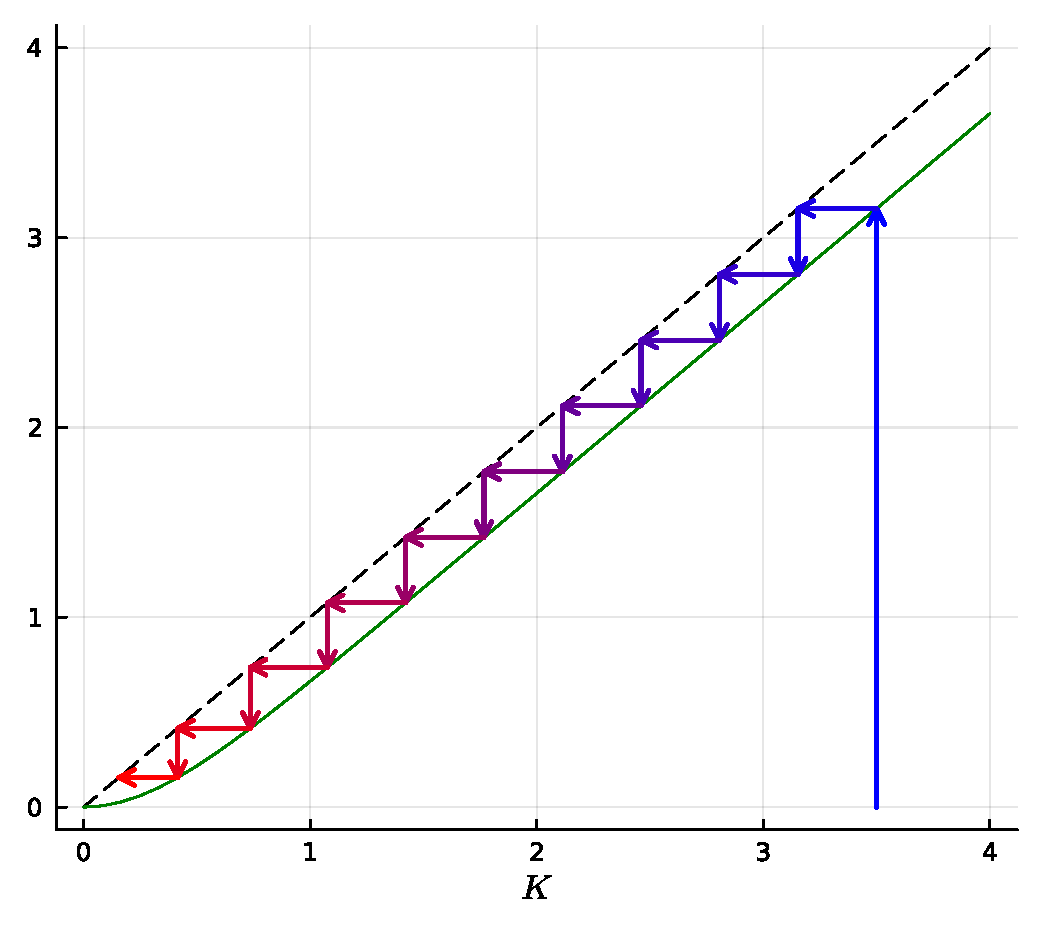
\includegraphics[width=0.56\textwidth]{codes/RG.pdf}
    \caption{\textbf{The decimation process.} Starting from $K\tund{0}=3.5$, we map it onto the curve $K'=\frac{1}{2}\ln \cosh 2K$ and repeat the process. The black dashed line represents $K'=K$ line while the green line represents $K'=\frac{1}{2}\ln \cosh 2K$ line. The process converges to $K^*=0$}
\end{figure}


